\section{Energy balance}
\label{sec:pumps:energy}

The pump absorbs the effective power $\power_e$, whereas the hydraulic
power $\power_p = \dens \grav \vFlow_p \dhead_p < \power_e$ due to
several losses in the pump. The latter can be organized in three
categories.
\begin{itemize}
\item \emph{organic losses} occur outside of the main flow path and
  reduce the hydraulic or indicated power $\power_i$ transferred to
  the fluid passing through the impeller.; they include
  \begin{itemize}
  \item the \emph{mechanical losses} $\power_m$ by friction in
    bearings, packings, \ldots;
  \item the \emph{disk friction losses} $\power_d$ due to
    recirculating flow in the (almost closed) cavity between the
    impeller and the housing.
  \end{itemize}
  The associated efficiency is the \emph{mechanical} or \emph{organic}
  efficiency, defined as the ratio of the power passed to the fluid to
  the total power input:
  \begin{align*}
    \eff_m 
    = \frac{\power_h}{\power_e} 
    = \frac{\power_e - \power_m - \power_d}{\power_e}
  \end{align*}
\item \emph{leakage losses} correspond to the (small) fraction of the
  total flow rate $\vFlow_i$ traversing the impeller that is
  subsequently recirculated to the inlet. Thereby it loses all of the
  energy it was given, including both mechanical and thermal energy,
  such that the associated power loss is
  \begin{align*}
    \power_l = \dens \grav \vFlow_l \dhead_i 
  \end{align*}
  The associated \emph{volumetric} efficiency also corresponds to the
  ratio of the effective pump flow rate to the impeller flow rate
  \begin{align*}
    \eff_v 
    = \frac{\dens \grav \vFlow_p \dhead_i}{\dens \grav \vFlow_i \dhead_i} 
    = \frac{\vFlow_p}{\vFlow_i} = \frac{\vFlow_i - \vFlow_l}{\vFlow_i}
  \end{align*}
\item \emph{hydrodynamic losses} occur along the flow path. A first
  type results in a reduction of the \emph{pump total head} $\dhead_p$
  with respect to the \emph{theoretical} or \emph{indicated head}
  $\dhead_i$. The nature of these losses was already discussed in the
  previous section. The \emph{indicated efficiency} corresponds to the
  useful head to the total energy given to the fluid:
  \begin{align*}
    \eff_i = \frac{\dhead_p}{\dhead_i}
  \end{align*}
\item \emph{recirculation losses} result from local recirculations in
  the vicinity of the impeller in- and/or outlet, occurring at lower
  flow rates. This recirculatory flow dissipates a pumping power
  $\power_r$; therefore the total hydraulic power is the sum of the
  indicated power and the recirculation power $\power_h = \power_i +
  \power_r$. We can associate an efficiency, relating to the total
  energy imparted to the fluid passing through the pump to the total
  hydraulic power
  \begin{align*}
    \eff_r = 
    \frac{\dens \grav \vFlow_i \dhead_i}{\dens \grav \vFlow_i \dhead_i + \power_r} = 
    \frac{\power_i}{\power_i + \power_r}
  \end{align*}
  The total hydraulic efficiency is then $\eff_h = \eff_i \cdot \eff_r$
\end{itemize}
The total power dissipated in the pump is then $\power_e = \power_m +
\dens \grav \vFlow_i \dhead_i + \power_r$, whereas the useful power is
$\power_p = \dens \grav \vFlow_p \dhead_p$. The global efficiency of
the pump is then
\begin{align*}
  \eff_p = 
  \frac{\dens \grav \vFlow_p \dhead_p}{\power_e} = 
  \frac{\power_h}{\power_e} \cdot 
  \frac{\power_i}{\power_h} \cdot 
  \frac{\dhead_p}{\dhead_i} \cdot 
  \frac{\vFlow_p}{\vFlow_i} 
  = \eff_m \cdot \eff_r \cdot \eff_i \cdot \eff_v
\end{align*}
In the next subsections we will briefly discuss the nature of the
losses except for the head losses, previously discussed in section
\ref{sec:pumps:head}.

%% -----------------------------------------------------------------------------
\subsection{Organic losses}
%% -----------------------------------------------------------------------------

Organic losses occur outside of the main flow path and are therefore
seen as reducing the power provided to the impeller instead of
directly extracting energy from the fluid. These include mechanical
and disk friction losses.

\subsubsection{Mechanical losses}

Mechanical losses result from friction in the bearings and the
packing; the latter is required to seal the pump flow path off from
the exterior. Mechanical losses are very difficult to measure since
they are very small: typically only up to a few percent of the total
power. As they occur outside of the pump, these are called
\emph{external organic losses}.

\subsubsection{Disk friction}

\begin{wrapfigure}{R}{0.34\textwidth}
  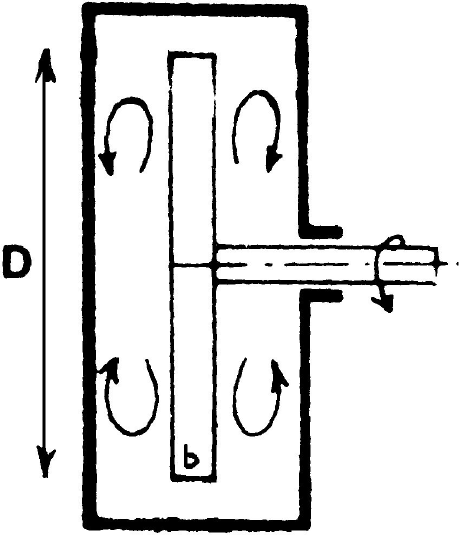
\includegraphics[width=0.34\textwidth]{pumps/diskFriction.png}
  \caption{Flow pattern between impeller disk and housing}
  \label{fig:diskFriction}
\end{wrapfigure} 
In radial and mixed flow pumps, a flow recirculation is generated in
the cavity between the impeller outer flasks and the housing. The
impeller outer surfaces entrain fluid particles in their rotating
motion, resulting in an outward centrifugal force. The resulting
secondary flow motion is sketched in figure \ref{fig:diskFriction}.

The energy dissipated by this recirculation is provided by the work
performed by the impeller outer surfaces. The local tangential
friction force on the disk is supposed to be proportional to the
rotational kinetic energy
\begin{align*}
  F_u = k \dens u^2 = k \dens \rot^2 R^2
\end{align*}
such that the contribution to the work of an annulus at radius R is 
\begin{align*}
  d M = 2 \pi R dR \cdot R \cdot F_u = 2 \pi k \rot^2 R^4 dR
\end{align*}
The corresponding power on one of the surfaces is
\begin{align*}
  \int_{R_1}^{R_2} 2 \pi k \rot^3 R^4 dR = \frac{2 \pi}{5} k \dens
  \rot^3 \left(R_2^5 - R_1^5\right) \approx \frac{2 \pi}{5} k \dens
  \rot^3 R_2^5
\end{align*}
The same reasoning can be applied to the rims of the impeller, which
can be simplified to a cylinder with combined height $b$ and radius
$R_2$; the corresponding power is
\begin{align*}
  2 \pi k \rot^3 R_2^4 b
\end{align*}
Since for both the front and the back of the impeller $R_1^5 <<
R_2^5$, the total power for a fully closed impeller finally is
\begin{equation}
  \power_f = 
  \frac{4 \pi}{5} k \dens \rot^3 R_2^5 
  \left(1+\frac{5}{2} \frac{b}{R_2}\right)
\end{equation}

The coefficient $k$ hides the effect of the flow pattern and needs to
be determined experimentally; it is a function of the fluid viscosity,
the surface roughness and finally the form of the cavity, in
particular the proximity of the casing. A commonly used value for
water and clean surfaces is $k=0.0012$. Improving the surface
roughness, \eg by painting or machining, can easily reduce these
losses by 20 to 30\%; since the contribution to the power increases
with $R^5$, it suffices to treat the outer parts of the impeller.

Since the friction is generated by fluid which remains mostly captured
in the cavity, the disk friction is considered as occurring outside of
the flow path, comparable to the mechanical losses; it is therefore
qualified as an \emph{internal organic loss}.

%% -----------------------------------------------------------------------------
\subsection{Leakage losses}
%% -----------------------------------------------------------------------------

\begin{figure}[!h]
  \centering {
    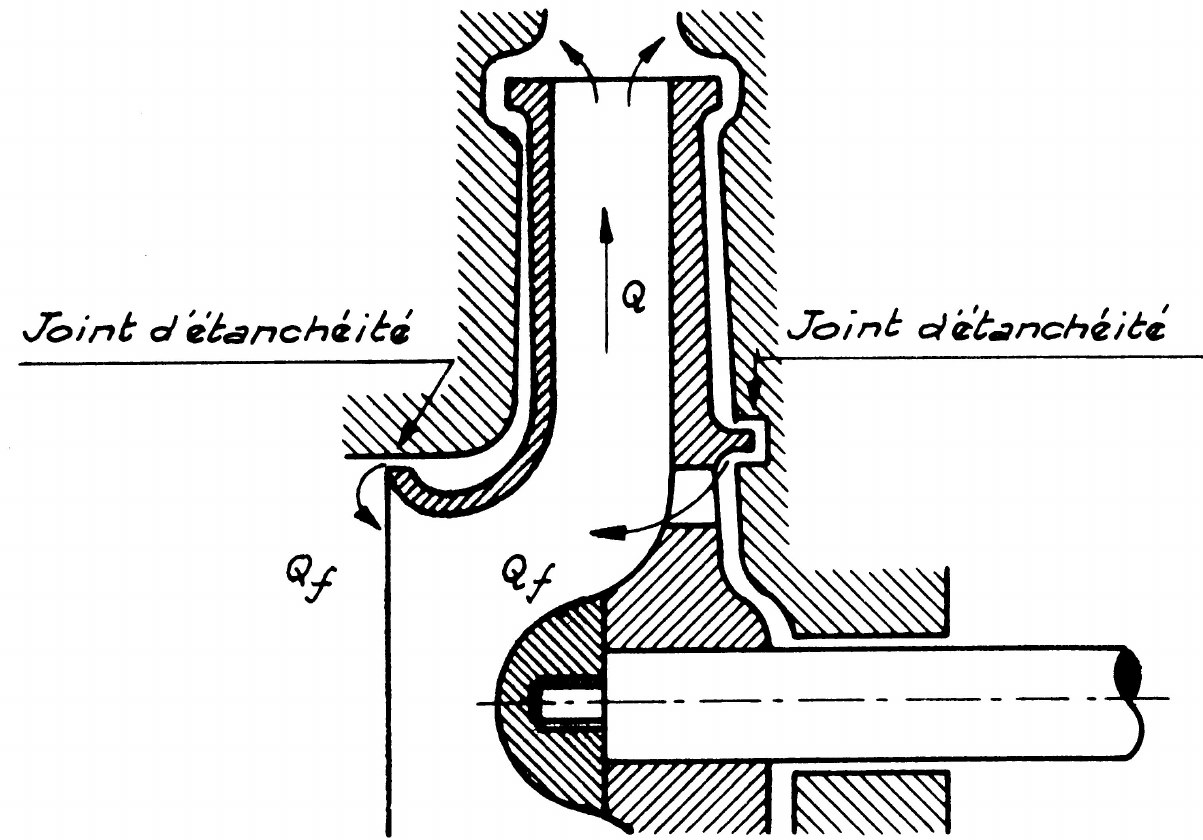
\includegraphics[width=0.5\textwidth]{pumps/leakagePaths.png}}
  \caption{Internal leakage paths through seals and balancing holes}
  \label{fig:leakagePaths}
\end{figure}

\subsubsection{External leakage flows - packings}

\todo{provide figure showing packings}
In order to reduce leakage out of the pump through the gap between the
rotating shaft and the casing of the pump, flexible rings or
\emph{packings} are axially compressed in a stuffing box surrounding
the shaft. The compression of these packings should be high enough to
stop or reduce leakage to acceptable levels, but not as high as to
prevent wetting of the packing, required to avoid overheating;
sometimes a controlled leakage is allowed for the most loaded packing.

\subsubsection{Internal leakage flows - seals}

\begin{figure}[!h]
  \centering{
    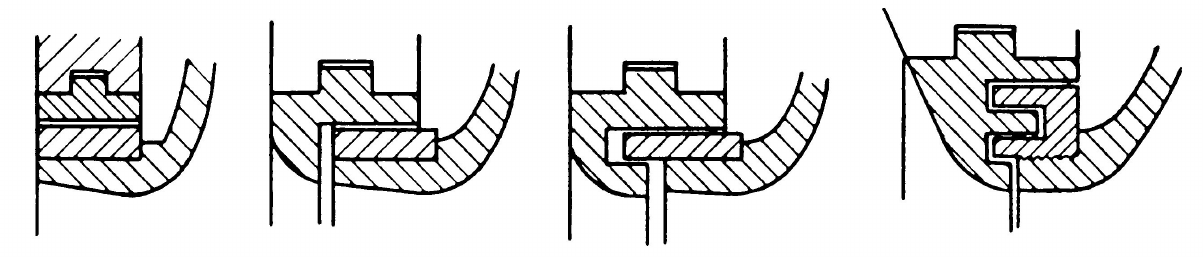
\includegraphics[width=\textwidth]{pumps/seals.png}
  }
  \caption{Seal types at the impeller eye: straight, abutted, abutted
    with one and three bends.}
  \label{fig:seals}
\end{figure}

Next to the external leakage, there are also important internal
leakage flows. A first category concerns flow through the gaps between
the impeller and the casing, leading the flow from the outlet back to
the inlet. These leakage flows are minimized through the use of seals,
illustrated in figure \ref{fig:seals}. The flow through the seals is
function of the pressure difference or head loss across the seal and
the (small) gap between the stationary and the rotating part. By
positioning the shroud seals close to the inlet, the pressure
difference can be minimized.

For the computation of the head loss, we apply the recipes in section
\ref{sec:pumps:hydraulicLosses}. It has three contributions, associated to
the entering of the flow in the annulus, with typical kinetic energy
factor $1/2$; the friction loss in the annulus, computed using the
Darcy-Weisbach correlations; and finally the discharge loss when
leaving the seal, in which the kinetic energy is fully lost. The head
loss is then a function of the bulk velocity $\vel_l$
\begin{align*}
  \loss_{seal} = \frac{1}{2} 
  \frac{\vel^2_l}{2g} + 
  \lambda \frac{L}{D_h} \frac{\vel^2_l}{2g} + 
  \frac{\vel^2_l}{2 g} = 
  \left(\frac{\lambda L}{D_h} + \frac{3}{2}\right) \frac{\vel^2}{2g}
\end{align*}
with $L$ the length of the seal, $D_h$ its equivalent hydraulic
diameter (approximately equal to half the gap $b$), and $\lambda$ the
friction coefficient. As before, $\lambda$ has to be determined
iteratively, as it depends on the flow velocity, but as a first
approximation $\lambda \approx 0.02 \ldots 0.03$.

This relation then allows us to compute the leakage flow rate by
equating the head loss in the flow through the seal to the head
difference over the seal:
\begin{align*}
  \vFlow_l = \frac{S}{\sqrt{\frac{\lambda L}{D_h} + \frac{3}{2}}} ~ 
  \frac{2 \Delta p}{\dens}
\end{align*}
In case the seal has $n$ bends, the flow rate can be similarly
computed as
\begin{align*}
  \vFlow_l = \frac{S}{\sqrt{\frac{\lambda L}{D_h} + \frac{3}{2} + n k_b}} ~ 
  \frac{2 \Delta p}{\dens}
\end{align*}
with $k_b$ the kinetic energy factor of a 180$^\circ$ bend and $L$ the
total length of the seal.

\subsubsection{Internal leakage flow - balancing holes} 

The hub back seal is positioned not only to minimize leakage, but also
to contribute to the axial balance of the pump. The pressure forces on
the impeller shroud and hub plate above the impeller eye radius can be
more more or less balanced; for this reason the hub back seal is often
more or less at the same radial position as the shroud/inlet seal.

On the other hand, the part of the hub cover lower than the inlet
radius has no counterpart on the shroud cover. The resulting axial
force is undesirable, and therefore sometimes \emph{balancing holes}
are foreseen to equalise the pressure across the hub cover as shown in
figure \ref{fig:leakagePaths}, thereby removing the resulting axial
thrust.

\subsection{Recirculation losses}

At flow rates $\vFlow_p$ much lower than the nominal one $\vFlow_p^n$,
recirculation occurs at in- and outlets of the impellers of both
centrifugal as well as axial pumps. The typical recirculation patterns
are sketched in figure \ref{fig:recirculationRadial} for both radial
and axial pumps.
\begin{figure}[!h]
  \begin{subfigure}{0.49\textwidth}
    \centering{
      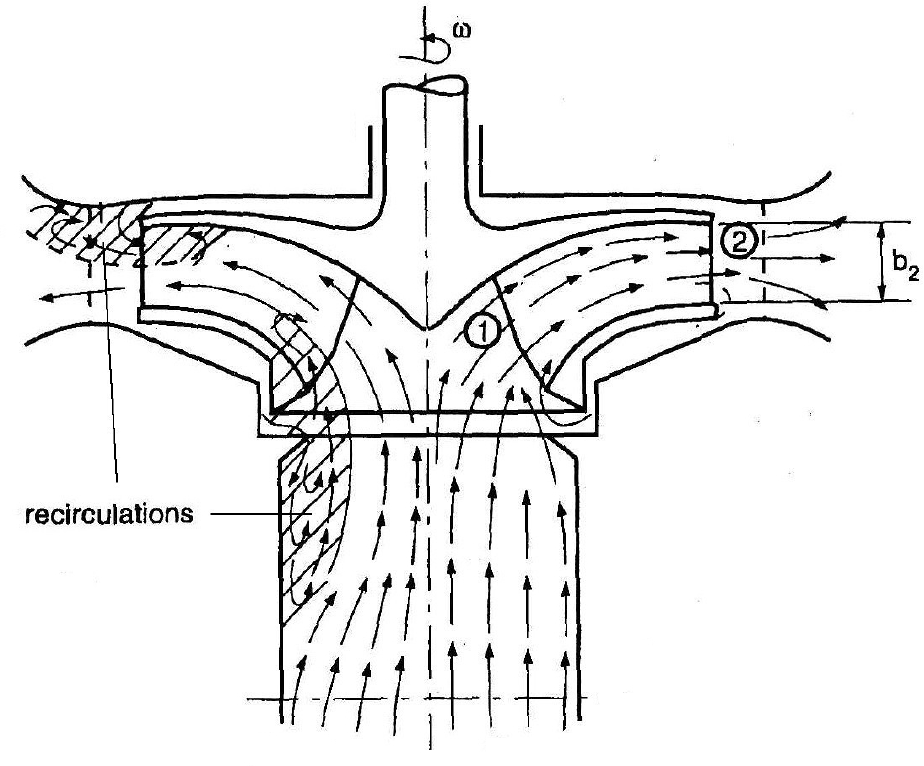
\includegraphics[width=\textwidth]{pumps/recirculationsRadial.png}}
    \caption{In radial pumps. \leonard.}
    \label{fig:recirculationRadial}
  \end{subfigure}
  \begin{subfigure}{0.49\textwidth}
    \centering{
      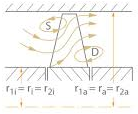
\includegraphics[width=\textwidth]{pumps/recirculationsAxial_KSB.png}}
    \caption{In axial pumps. Reproduced
      from \cite{KSB}.}
    \label{fig:recirculationAxial}
  \end{subfigure}
  \caption{Recirculation patterns occuring at low flow rate.}
  \label{fig:recirculations}
\end{figure}

The recirculation at the inlet of the impeller has similar origins for
radial and axial pumps. The flow entering the impeller has very high
incidence on the blade; the sudden change in flow direction results in
a very circumferential velocities, a rapid local increase of the total
and static head, and a very high radial pressure gradient, pushing the
flow upstream along the outer radius of the suction pipe. In case of
an unshrouded impeller, the very high pressure jump over the blade tip
results in a forward directed tip leakage flows pointing upstream. The
resulting upstream moving flow has significant circumferential
velocities and total pressure, to the point that the measurement of
the inlet static head may be compromised - it happens that the static
head at the wall exceeds the suction total dynamic head.

The recirculation patterns at the discharge side are obviously
different for radial and axial pumps. It results from the spanwise
concentration of the mass flow over part of the blade height. For
axial pumps, the radial pressure gradient due to the outlet swirl
ensures that the flow at the blade tip is forward and separation
happens at the root. For a radial pump, the location depends on the
(secondary) flow in the impeller and the downstream diffuser.

The energy dissipated in the recirculation flows can represent a very
significant part of the total power. Its value depends on the geometry
of the machine and varies approximately as 
\begin{align*}
  \power_r = k_r \left(1 - \frac{\vFlow_p}{\vFlow_p^n}\right)^2
\end{align*}
The limiting flow rate at which recirculation appears depends on many
parameters, in particular the type of pump and its specific speed. The
values may even be different for inlet and discharge
recirculation. For a typical centrifugal pump, the critical flow rate
varies from $0.5$ to $0.8 \vFlow_p^n$. In general, its occurence and
consequences are more pronounced for axial pumps than for radial.



%%% Local Variables: 
%%% mode: latex
%%% TeX-master: "../MECA0467"
%%% End: 
